\def\documentauthor{Carlos Salinas}
\def\documenttitle{MA 166: Quiz \hwnum}
\def\hwnum{3}
\def\shorttitle{MA 166 HW \hwnum}
\def\coursename{MA166}
\def\documentsubject{calculus ii}
\def\authoremail{salinac@purdue.edu}

\documentclass[12pt]{article}
\usepackage{geometry}
\usepackage[dvipsnames]{xcolor}
\usepackage[
    breaklinks,
    bookmarks=true,
    colorlinks=true,
    pageanchor=false,
    linkcolor=black,
    anchorcolor=black,
    citecolor=black,
    filecolor=black,
    menucolor=black,
    runcolor=black,
    urlcolor=black,
    hyperindex=false,
    hyperfootnotes=true,
    pdftitle={\shorttitle},
    pdfauthor={\documentauthor},
    pdfkeywords={\documentsubject},
    pdfsubject={\coursename}
    ]{hyperref}

% Use symbols instead of numbers
\renewcommand*{\thefootnote}{\fnsymbol{footnote}}

%% Math
\usepackage{amsmath}
\usepackage{amsthm}
\usepackage{amssymb}
\usepackage{mathtools}

%%PDFTeX specific
\usepackage[mathcal]{euscript}
\usepackage{mathrsfs}
\usepackage{dsfont}
\usepackage{wasysym}

\usepackage[LAE,LFE,T2A,T1]{fontenc}
\usepackage[utf8]{inputenc}
\usepackage[farsi,french,german,spanish,russian,english]{babel}
\babeltags{pa=farsi,
           fr=french,
           de=german,
           es=spanish,
           ru=russian,
           en=english}
\def\spanishoptions{mexico}

\selectlanguage{english}

\newcommand{\textfa}[1]{\beginR\textpa{#1}\endR}

\usepackage{cmap}
\usepackage{CJKutf8}
\newcommand{\textkr}[1]{\begin{CJK}{UTF8}{mj}#1\end{CJK}}
\newcommand{\textjp}[1]{\begin{CJK}{UTF8}{min}#1\end{CJK}}
\newcommand{\textzh}[1]{\begin{CJK}{UTF8}{bsmi}#1\end{CJK}}

%% Misc
\usepackage{graphicx}
\usepackage{cutwin}
\graphicspath{{figures/}}

\usepackage{microtype}
\usepackage{multicol}
\usepackage[inline]{enumitem}
\usepackage{listings}
\usepackage{mleftright}
\mleftright

%% Theorems and definitions
\theoremstyle{plain}
\newtheorem{theorem}{Theorem}
\newtheorem{proposition}[theorem]{Proposition}
\newtheorem{corollary}[theorem]{Corollary}
\newtheorem{claim}[theorem]{Claim}
\newtheorem{lemma}[theorem]{Lemma}
\newtheorem{axiom}[theorem]{Axiom}

\newtheorem*{corollary*}{Corollary}
\newtheorem*{claim*}{Claim}
\newtheorem*{lemma*}{Lemma}
\newtheorem*{proposition*}{Proposition}
\newtheorem*{theorem*}{Theorem}

\theoremstyle{definition}
\newtheorem{definition}{Definition}
\newtheorem{example}{Examples}
\newtheorem{examples}[example]{Examples}
\newtheorem{exercise}{Exercise}
\newtheorem{problem}[exercise]{Problem}

\newtheorem*{definition*}{Definition}
\newtheorem*{example*}{Examples}
\newtheorem*{examples*}{Examples}
\newtheorem*{exercise*}{Exercise}
\newtheorem*{problem*}{Problem}

\theoremstyle{remark}
\newtheorem{remark}{Remark}
\newtheorem{remarks}[remark]{Remarks}
\newtheorem{observation}[remark]{Observation}
\newtheorem{observations}[remark]{Observations}

\newtheorem*{remark*}{**Remark**}
\newtheorem*{remarks*}{**Remarks**}
\newtheorem*{observation*}{**Observation**}
\newtheorem*{observations*}{**Observations**}

%% Commands and operators
%% Redefinitions & commands
\newcommand{\nsubset}{\ensuremath{\not\subset}}
\newcommand{\nsupset}{\ensuremath{\not\supset}}
\newcommand\minus{\ensuremath{\null\smallsetminus}}
\renewcommand\qedsymbol{\ensuremath{\null\hfill\blacksquare}}

%% Commands and operators
\DeclareMathOperator{\id}{id}
\DeclareMathOperator{\im}{im}

%% Linear algebra
\DeclareMathOperator{\proj}{proj}
\DeclareMathOperator{\comp}{comp}

%% Differential operators
\DeclareMathOperator{\Curl}{curl}
\DeclareMathOperator{\Div}{div}
\DeclareMathOperator{\Grad}{grad}
\DeclareMathOperator{\Lap}{\Delta}
\DeclareMathOperator{\diff}{d\!}

%% Misc
\newcommand{\bbC}{\mathbb{C}}
\newcommand{\bbCP}{\mathbb{CP}}
\newcommand{\bbH}{\mathbb{H}}
\newcommand{\bbN}{\mathbb{N}}
\newcommand{\bbQ}{\mathbb{Q}}
\newcommand{\bbR}{\mathbb{R}}
\newcommand{\bbRP}{\mathbb{RP}}
\newcommand{\bbZ}{\mathbb{Z}}

\newcommand{\bfC}{\mathbf{C}}
\newcommand{\bfCP}{\mathbf{CP}}
\newcommand{\bfH}{\mathbf{H}}
\newcommand{\bfN}{\mathbf{N}}
\newcommand{\bfQ}{\mathbf{Q}}
\newcommand{\bfR}{\mathbf{R}}
\newcommand{\bfRP}{\mathbf{RP}}
\newcommand{\bfZ}{\mathbf{Z}}

\newcommand{\calA}{\mathcal{A}}
\newcommand{\calB}{\mathcal{B}}
\newcommand{\calC}{\mathcal{C}}
\newcommand{\calS}{\mathcal{S}}
\newcommand{\calT}{\mathcal{T}}
\newcommand{\calU}{\mathcal{U}}
\newcommand{\calV}{\mathcal{V}}

\newcommand{\scrL}{\mathscr{L}}
\newcommand{\scrO}{\mathscr{O}}
\newcommand{\scrS}{\mathscr{S}}

\newcommand{\bfa}{\mathbf{a}}
\newcommand{\bfb}{\mathbf{b}}
\newcommand{\bfc}{\mathbf{c}}
\newcommand{\bfu}{\mathbf{u}}
\newcommand{\bfv}{\mathbf{v}}
\newcommand{\bfw}{\mathbf{w}}

\begin{document}
\author{TA: \href{mailto:\authoremail}{\documentauthor}}
\title{\documenttitle}
\date{\today}
\maketitle

You have \textbf{15 minutes} to complete this quiz. You may work in groups,
but you are not allowed to use any other resources.
\\\\
%% Quiz problems
% \begin{problem}[Easy]
% Shown is the graph of a force function (in Newtons) that increases to its
% maximum value and then remains constant. How much work $W$ is done by the
% force in moving an object a distance of $24$ meters?
% \begin{center}
% 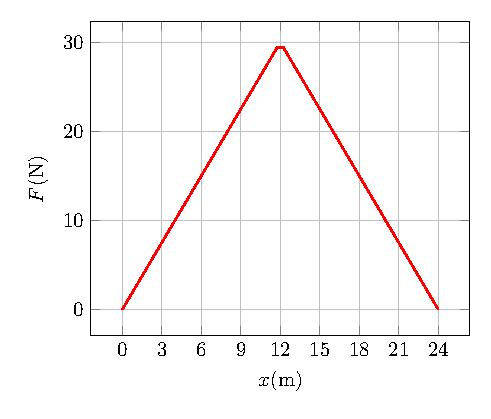
\includegraphics[scale=0.75]{../figures/quiz-4-fig-1}
% \end{center}
% \end{problem}
\begin{problem}[Medium]
\begin{enumerate}[label=(\alph*)]
\item Find the volume $V$ of the solid obtained by rotating the region
  enclosed by the curves $y=x^2$ and $y=x^3$ about the $x$-axis.
\item The region inside the circle $x^2+y^2=1$ and to the right of the line
  $x=1/2$ is rotated about the $y$-axis. Use the method of shells to find
  the volume of the resulting solid.
\item Find the indefinite integral
\[
\int x^5e^{-x}\diff x.
\]
\end{enumerate}
\end{problem}
\begin{problem}
  The tank pictured below is full of water. Let $a=6$, $b=4$, and $c=8$. Do
  not worry about the spout. Set up the integral which gives the work
  required to pump all of the water over the top. Do not evaluate the
  integral. (Water weighs $62.5$ lbs/ft$^3$, accounting for gravity).
\begin{center}
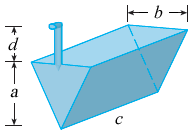
\includegraphics[scale=0.5]{../figures/hw-7-fig-2}
\end{center}
\end{problem}
\begin{problem}
A solid $S$ has a square base on the $xy$-plane with four points $(1,0)$,
$(0,1)$, $(-1,0)$ and $(0,-1)$ as vertices. Its cross-section perpendicular
to the $x$-axis are equilateral triangles. Find an expression for the
volume of $S$.
\end{problem}
\end{document}

%%% Local Variables:
%%% mode: latex
%%% TeX-master: t
%%% End:
